
\subsection{Explotar o seguir explorando}\label{subsection:exp-epsilon}

En esta sección se muestran los experimentos para comparar
el desempeño de los algoritmos con dos valores diferentes para
el factor que controla la tasa de decremento de $\epsilon$. El primer valor 
es bajo, para dejar de dar peso a la exploración después del primer
cuarto de entrenamiento y el segundo es alto, para llegar a una máxima probabilidad
de explotación en el último cuarto del aprendizaje.

\subsubsection{Configuración experimental}

\begin{itemize}
    \item El espacio de estados es discreto, es decir, el agente puede
    obtener las variables $\mathcal{X}$ directamente del ambiente.
    \item Para obtener a los
    grafos $\mathcal{D'}$ y $\mathcal{D''}$,
    el porcentaje de nivel de cambio  es $p_{mod} = 25 \%$. Esto significa que no se altera demasiado el grafo causal original para
    generar los grafos incompletos e incorrectos.
    \item Se controla qué tan rápido se desea alcanzar $\epsilon_{\min}$ variando el parámetro $\delta$. Si se divide al entrenamiento en cuartos,  entonces los valores de $\delta$ corresponden a en qué cuarto se alcanza el mínimo valor para $\epsilon$.
    \begin{itemize}
        \item Alcanzar $\epsilon_{\min}$ en el primer cuarto del entrenamiento, $\delta = 0.25$.
        \item Alcanzar $\epsilon_{\min}$ a medio aprendizaje, $\delta = 0.50$.
        \item Alcanzar $\epsilon_{\min}$ en el tercer cuarto del entrenamiento, $\delta = 0.75$.
    \end{itemize}
    \item Se examina sobre los tres tipos de estructuras posibles: uno-a-uno, 
    causa común y efecto común. 
    \item Se prueba sobre un mundo determinista y uno estocástico.
    \item Dado que en la sección \ref{exp1}, $\delta=0.5$, este valor se deja fuera para estos experimentos.
\end{itemize}

\subsubsection{Objetivo}

Determinar si reducir o aumentar las consultas al grafo causal a lo largo del aprendizaje afecta el desempeño
de los algoritmos.

\subsubsection{Hipótesis}

La información del grafo causal no afecta negativamente 
el aprendizaje de la función de valor $Q$. Por lo tanto, incluso si se disminuyen las consultas al modelo de manera temprana en el entrenamiento, la información provista habrá
ayudado al aprendizaje de la función de valor.

\subsubsection{Resultados}

A fin de  comparar el desempeño de los algoritmos
para las diferentes configuraciones del experimento
se evalúa la medida \textit{average}.
De manera gráfica, se muestra el desempeño de los algoritmos
para los diferentes valores $\delta$ en las Figuras \ref{fig:low-epsilon-det}, \ref{fig:low-epsilon-sto}, \ref{fig:high-epsilon-det} y \ref{fig:high-epsilon-sto}.

En las Figuras \ref{fig:low-epsilon-det}-\ref{fig:high-epsilon-sto} se puede ver que en la mayoría de los casos, los algoritmos que utilizan conocimiento del grafo inician con una recompensa mayor y se estabilizan más rápido que el algoritmo Q-learning
sin información adicional en ambientes con transiciones deterministas y estocásticas.
De acuerdo con los resultados parece que 
entre mayor sea $\delta$ más tarda en estabilizarse
el algoritmo de aprendizaje sin información que lo auxilie. Esto es de esperarse, ya que se sigue explorando durante más tiempo. 
Por otro lado, para las estructuras uno-a-uno, la recompensa en los algoritmos que se guían por el grafo, se desestabiliza el intervalo en el que se encuentra la transición a dejar de dar peso a
la exploración. Pero, una vez fuera de esa ``zona de transición'' los
algoritmos se recuperan y tienden a estar por encima del algoritmo sin datos 
extra.

Por otro lado, además de las curvas de aprendizaje se propone hacer una comparación estadística de
los métodos. Para esto, se
compara la recompensa promedio de los últimos $E$ episodios
de entrenamiento sobre los $M$ experimentos. Con esto, se 
puede obtener una muestra de tamaño $E$ para cada algoritmo
y hacer una prueba estadística para mostrar que existe una diferencia entre ellos. La prueba estadística se realiza comparando los algoritmos que utilizan información extra versus el algoritmo Q-learning usando una exploración a prueba y error para saber si los primeros son superiores significativamente sobre el segundo. 

En las tablas \ref{tab:delta-one-to-one}, \ref{tab:delta-one-to-many} y \ref{tab:delta-many-to-one} se muestran
los promedios de las recompensas durante los últimos $E$ episodios. 
De igual manera que en las curvas de aprendizaje se puede notar que en la mayoría de tareas el algoritmo Q-learning usando el grafo causal completo tiene una recompensa mayor que en los otros métodos. Además, en general los métodos que utilizan el grafo ya sea incorrecto o incompleto superan al método clásico de Q-learning. Para validar estos resultados se usa la prueba de Welch con $p < 0.05$ para encontrar diferencias estadísticamente significativas. 
Los resultados de las pruebas refuerzan lo concluido a partir de las gráficas. Existe una diferencia estadística en el desempeño de los algoritmos, excepto por algunos casos (marcados por $\dagger$ en las tablas). Estos últimos corresponden
al desempeño en tareas con una estructura causal subyacente de tipo uno a uno y con $N=9$. Esto puede ser debido a esta transición
de exploración y explotación. 

\begin{table}[h]
\centering
\caption{Comparación de la recompensa promedio obtenida durante los últimos $E=100$ episodios de entrenamiento para $M$ experimentos en tareas con estructuras causales uno a uno.}
\label{tab:delta-one-to-one}
\resizebox{\textwidth}{!}{%
\begin{tabular}{@{}ccclll@{}}
\toprule
Ambiente & $\delta$ & Algoritmo & \multicolumn{3}{c}{$N$} \\ \cmidrule(l){4-6} 
 &  &  & \multicolumn{1}{c}{5} & \multicolumn{1}{c}{7} & \multicolumn{1}{c}{9} \\ \midrule
Determinista & $0.25$ & $Q_{1}$ & $-2.2324 \pm 0.6353$ & $-4.3184 \pm 0.8746$ & $-6.3564 \pm 1.3603$ \\
 &  & $Q_{2}$ & $\mathbf{-1.9466 \pm 0.4679}$ & $-3.5731 \pm 0.7285$ & $-5.7115 \pm 1.1855$ \\
 &  & $Q_{2}$ & $-1.9825 \pm 0.4632$ & $\mathbf{-3.5061 \pm 0.7207}$ & $\mathbf{-5.6209 \pm 1.0718}$ \\
 &  & $Q_{4}$ & $-2.0330 \pm 0.5384$ & $-3.5547 \pm 0.7081$ & $-5.8372 \pm 1.0747$ \\ \cmidrule(l){2-6} 
 & $0.75$ & $Q_{1}$ & $-2.3774 \pm 0.6925$ & $-4.3218 \pm 0.9312$ & $-6.2775 \pm 1.1195$ \\
 &  & $Q_{2}$ & $\mathbf{-1.8880 \pm 0.4666}$ & $\mathbf{-3.4929 \pm 0.7115}$ & $-6.9414 \pm 1.6493$ \\
 &  & $Q_{2}$ & $-2.1314 \pm 0.4933$ & $-3.8299 \pm 0.7694$ & $-6.3671 \pm 1.4099\dagger$ \\
 &  & $Q_{4}$ & $-1.9896 \pm 0.5470$ & $-3.8252 \pm 0.7840$ & $\mathbf{-6.2538 \pm 1.3547\dagger}$ \\ \cmidrule(l){2-6} 
Estocástico & $0.25$ & $Q_{1}$ & $-4.8575 \pm 0.9453$ & $-9.3174 \pm 1.2780$ & $-14.5087 \pm 1.4934$ \\
 &  & $Q_{2}$ & $\mathbf{-3.4833 \pm 0.8100}$ & $-7.2904 \pm 1.3719$ & $\mathbf{-10.7682 \pm 1.8282}$ \\
 &  & $Q_{2}$ & $-3.7870 \pm 0.8263$ & $\mathbf{-6.8757 \pm 1.2246}$ & $-11.9817 \pm 1.9420$ \\
 &  & $Q_{4}$ & $-3.8850 \pm 0.8119$ & $-7.1184 \pm 1.1471$ & $-12.4496 \pm 1.9692$ \\ \cmidrule(l){2-6} 
 & $0.75$ & $Q_{1}$ & $-5.0956 \pm 0.8950$ & $-9.3535 \pm 1.2484$ & $-14.3432 \pm 1.7236$ \\
 &  & $Q_{2}$ & $\mathbf{-3.9598 \pm 0.8291}$ & $-8.1395 \pm 1.3979$ & $\mathbf{-13.7784 \pm 1.8453}$ \\
 &  & $Q_{2}$ & $-4.2412 \pm 0.9166$ & $-8.4381 \pm 1.4981$ & $-13.8170 \pm 2.0379\dagger$ \\
 &  & $Q_{4}$ & $-3.9809 \pm 0.8148$ & $\mathbf{-8.1071 \pm 1.2102}$ & $-13.9492 \pm 1.7832\dagger$ \\ \bottomrule
\end{tabular}%
}
\end{table}

\newpage

\begin{table}[]
\centering
\caption{Comparación de la recompensa promedio obtenida durante los últimos $E=100$ episodios de entrenamiento para $M$ experimentos en tareas con estructuras de causa común.}
\label{tab:delta-one-to-many}
\resizebox{\textwidth}{!}{%
\begin{tabular}{ccclll}
\hline
Ambiente & $\delta$ & Algoritmo & \multicolumn{3}{c}{$N$} \\ \cline{4-6} 
 &  &  & \multicolumn{1}{c}{5} & \multicolumn{1}{c}{7} & \multicolumn{1}{c}{9} \\ \hline
Determinista & $0.25$ & $Q_{1}$ & $-1.1242 \pm 0.4301$ & $-2.4038 \pm 0.7038$ & $-2.9975 \pm 0.8161$ \\
 &  & $Q_{2}$ & $-0.8281 \pm 0.2998$ & $\mathbf{-1.8221 \pm 0.5187}$ & $\mathbf{-2.4173 \pm 0.5790}$ \\
 &  & $Q_{2}$ & $-0.8161 \pm 0.2827$ & $-1.8789 \pm 0.4548$ & $-2.5532 \pm 0.5628$ \\
 &  & $Q_{4}$ & $\mathbf{-0.8068 \pm 0.3186}$ & $-1.8897 \pm 0.4411$ & $-2.5236 \pm 0.6685$ \\ \cline{2-6} 
 & $0.75$ & $Q_{1}$ & $-1.6430 \pm 0.6236$ & $-2.9379 \pm 0.7767$ & $-4.1146 \pm 1.2066$ \\
 &  & $Q_{2}$ & $\mathbf{-0.9273 \pm 0.2693}$ & $\mathbf{-1.6828 \pm 0.4610}$ & $\mathbf{-2.6278 \pm 0.6338}$ \\
 &  & $Q_{2}$ & $-1.0958 \pm 0.4066$ & $-1.9402 \pm 0.6138$ & $-2.9660 \pm 0.6821$ \\
 &  & $Q_{4}$ & $-1.0778 \pm 0.3990$ & $-1.9267 \pm 0.5551$ & $-3.3222 \pm 0.8773$ \\ \cline{2-6} 
Estocástico & $0.25$ & $Q_{1}$ & $-2.8257 \pm 0.8804$ & $-6.0498 \pm 1.4224$ & $-8.9472 \pm 1.7429$ \\
 &  & $Q_{2}$ & $\mathbf{-2.1866 \pm 0.7467}$ & $\mathbf{-4.0352 \pm 1.0788}$ & $\mathbf{-5.0238 \pm 1.3692}$ \\
 &  & $Q_{2}$ & $-2.2934 \pm 0.7969$ & $-4.0734 \pm 1.2090$ & $-5.3714 \pm 1.4905$ \\
 &  & $Q_{4}$ & $-2.2001 \pm 0.7131$ & $-4.2083 \pm 1.1122$ & $-5.4152 \pm 1.5542$ \\ \cline{2-6} 
 & $0.75$ & $Q_{1}$ & $-3.3176 \pm 1.0664$ & $-6.3604 \pm 1.4621$ & $-9.7091 \pm 1.8713$ \\
 &  & $Q_{2}$ & $\mathbf{-2.0068 \pm 0.6758}$ & $\mathbf{-4.1851 \pm 1.0592}$ & $\mathbf{-5.7100 \pm 1.5696}$ \\
 &  & $Q_{2}$ & $-2.2042 \pm 0.7600$ & $-4.5311 \pm 1.2282$ & $-6.8496 \pm 1.5566$ \\
 &  & $Q_{4}$ & $-2.3583 \pm 0.7962$ & $-4.6244 \pm 1.2486$ & $-6.3323 \pm 1.6861$ \\ \hline
\end{tabular}%
}
\end{table}

\begin{table}[]
\centering
\caption{Comparación de la recompensa promedio obtenida durante los últimos $E=100$ episodios de entrenamiento para $M$ experimentos en tareas con estructuras con relaciones de efecto común.}
\label{tab:delta-many-to-one}
\resizebox{\textwidth}{!}{%
\begin{tabular}{ccclll}
\hline
Ambiente & $\delta$ & Algoritmo & \multicolumn{3}{c}{$N$} \\ \cline{4-6} 
 &  &  & \multicolumn{1}{c}{5} & \multicolumn{1}{c}{7} & \multicolumn{1}{c}{9} \\ \hline
Determinista & $0.25$ & $Q_{1}$ & $-0.9308 \pm 0.3887$ & $-2.0693 \pm 0.6689$ & $-2.9613 \pm 0.7537$ \\
 &  & $Q_{2}$ & $\mathbf{-0.6354 \pm 0.2388}$ & $\mathbf{-1.5994 \pm 0.4242}$ & $-2.5653 \pm 0.5053$ \\
 &  & $Q_{2}$ & $-0.7521 \pm 0.2444$ & $-1.6121 \pm 0.4051$ & $\mathbf{-2.5128 \pm 0.5890}$ \\
 &  & $Q_{4}$ & $-0.6659 \pm 0.2323$ & $-1.5995 \pm 0.4407$ & $-2.6478 \pm 0.6228$ \\ \cline{2-6} 
 & $0.75$ & $Q_{1}$ & $-1.5390 \pm 0.5056$ & $-2.9007 \pm 0.7137$ & $-3.9921 \pm 1.0301$ \\
 &  & $Q_{2}$ & $\mathbf{-0.8006 \pm 0.2368}$ & $\mathbf{-1.7237 \pm 0.4467}$ & $\mathbf{-2.4808 \pm 0.5215}$ \\
 &  & $Q_{2}$ & $-0.9448 \pm 0.3327$ & $-1.9036 \pm 0.5026$ & $-2.8287 \pm 0.7198$ \\
 &  & $Q_{4}$ & $-0.8983 \pm 0.3522$ & $-1.7377 \pm 0.4231$ & $-2.9039 \pm 0.7814$ \\ \cline{2-6} 
Estocástico & $0.25$ & $Q_{1}$ & $-2.7417 \pm 0.8380$ & $-5.2262 \pm 1.1446$ & $-7.6755 \pm 1.5417$ \\
 &  & $Q_{2}$ & $-2.0551 \pm 0.6530$ & $-3.6230 \pm 1.0363$ & $\mathbf{-4.4380 \pm 1.1340}$ \\
 &  & $Q_{2}$ & $-2.0618 \pm 0.5730$ & $\mathbf{-3.3963 \pm 0.8821}$ & $-4.7390 \pm 1.1393$ \\
 &  & $Q_{4}$ & $\mathbf{-1.9463 \pm 0.6109}$ & $-3.6499 \pm 1.0723$ & $-5.6039 \pm 1.3790$ \\ \cline{2-6} 
 & $0.75$ & $Q_{1}$ & $-2.7992 \pm 0.8305$ & $-5.6699 \pm 1.3177$ & $-7.7359 \pm 1.7315$ \\
 &  & $Q_{2}$ & $\mathbf{-1.6935 \pm 0.5582}$ & $\mathbf{-3.7668 \pm 1.1628}$ & $\mathbf{-5.0338 \pm 1.0605}$ \\
 &  & $Q_{2}$ & $-1.8176 \pm 0.6096$ & $-4.0601 \pm 1.0350$ & $-5.9173 \pm 1.3811$ \\
 &  & $Q_{4}$ & $-2.2837 \pm 0.6340$ & $-4.5129 \pm 1.0016$ & $-5.6167 \pm 1.5121$ \\ \hline
\end{tabular}%
}
\end{table}

\newpage

\begin{figure}
\settoheight{\tempdima}{\includegraphics[width=.32\linewidth]{example-image-a}}%
\centering\begin{tabular}{@{}c@{ }c@{ }c@{ }c@{}}
&\textbf{Uno-a-uno} & \textbf{Causa común} & \textbf{Efecto común} \\
\rowname{$N = 5$}&
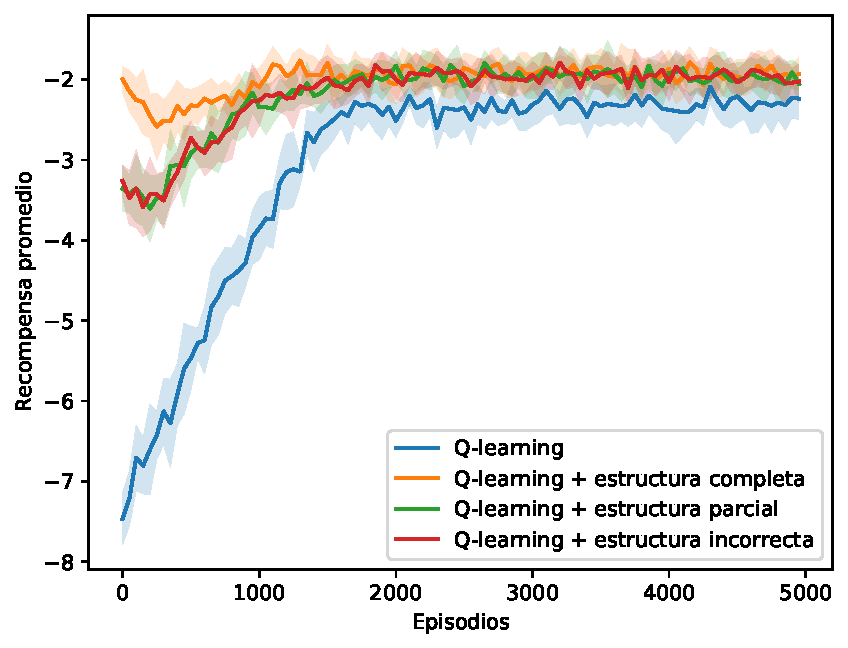
\includegraphics[width=.32\linewidth]{Chapter5/Figs/deltaexp/deterministic_low_025_one_to_one_N_5_experiments_10_episodes_5000_eps_6250.pdf}&
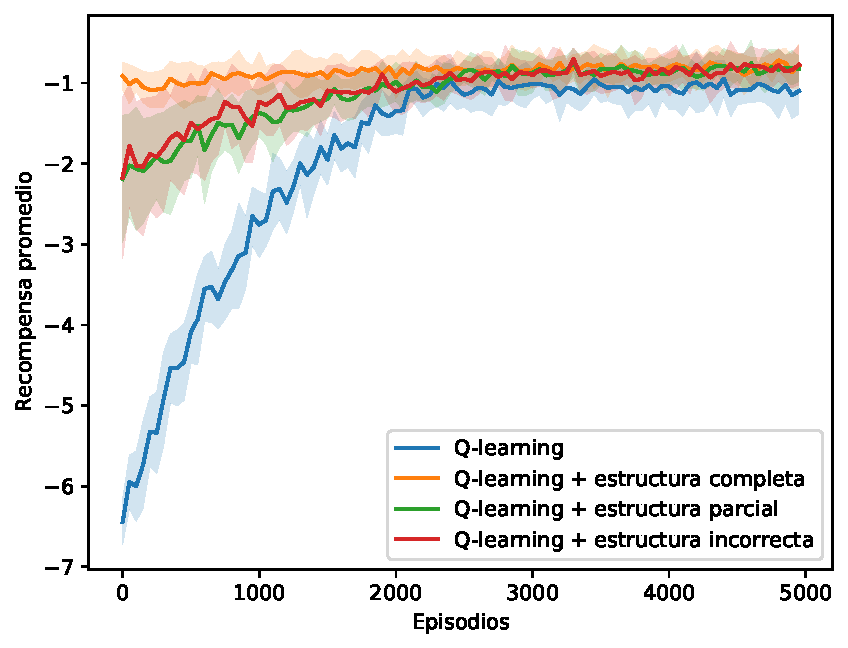
\includegraphics[width=.32\linewidth]{Chapter5/Figs/deltaexp/deterministic_low_025_one_to_many_N_5_experiments_10_episodes_5000_eps_6250.pdf}&
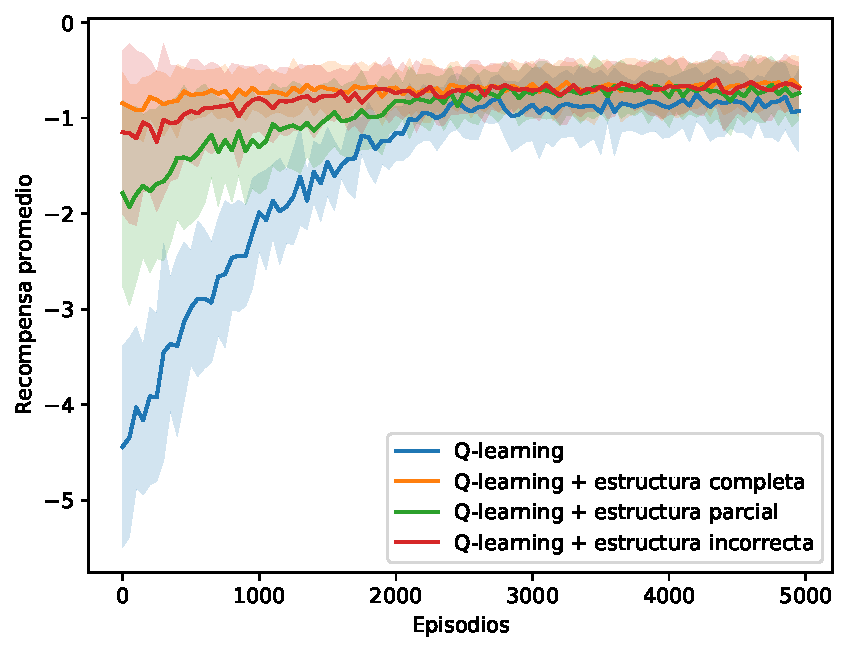
\includegraphics[width=.32\linewidth]{Chapter5/Figs/deltaexp/deterministic_low_025_many_to_one_N_5_experiments_10_episodes_5000_eps_6250.pdf}\\
\rowname{$N=7$}&
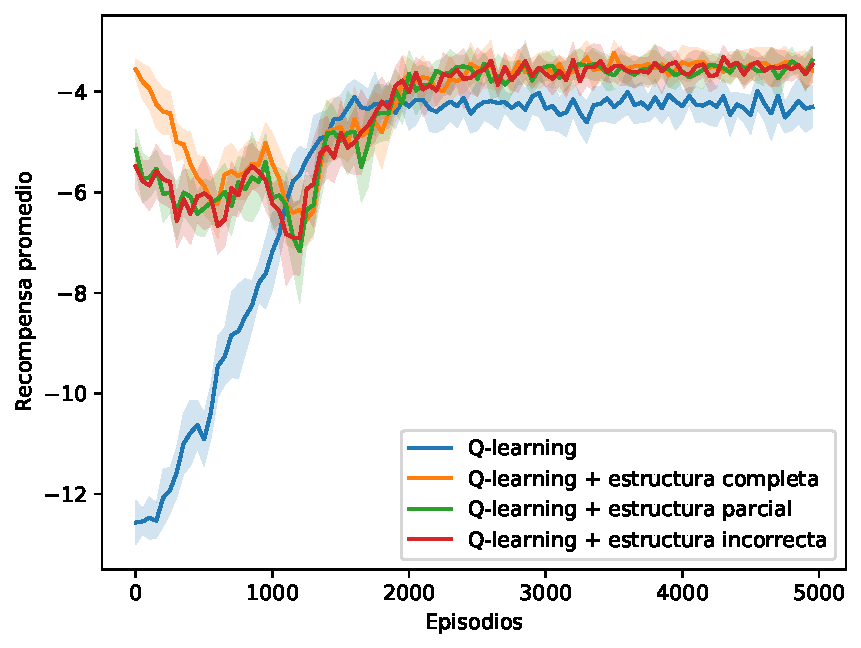
\includegraphics[width=.32\linewidth]{Chapter5/Figs/deltaexp/deterministic_low_025_one_to_one_N_7_experiments_10_episodes_5000_eps_8750.pdf}&
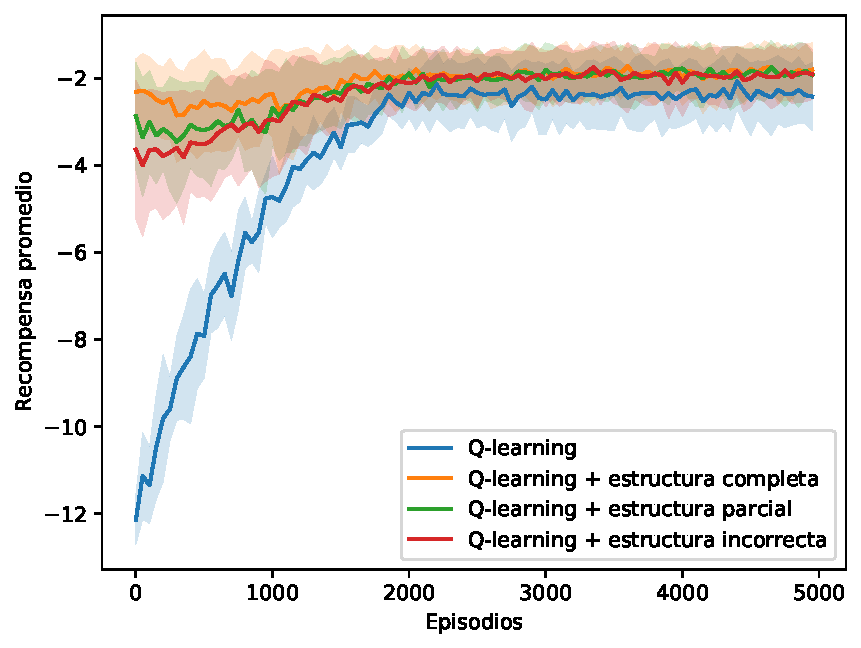
\includegraphics[width=.32\linewidth]{Chapter5/Figs/deltaexp/deterministic_low_025_one_to_many_N_7_experiments_10_episodes_5000_eps_8750.pdf}&
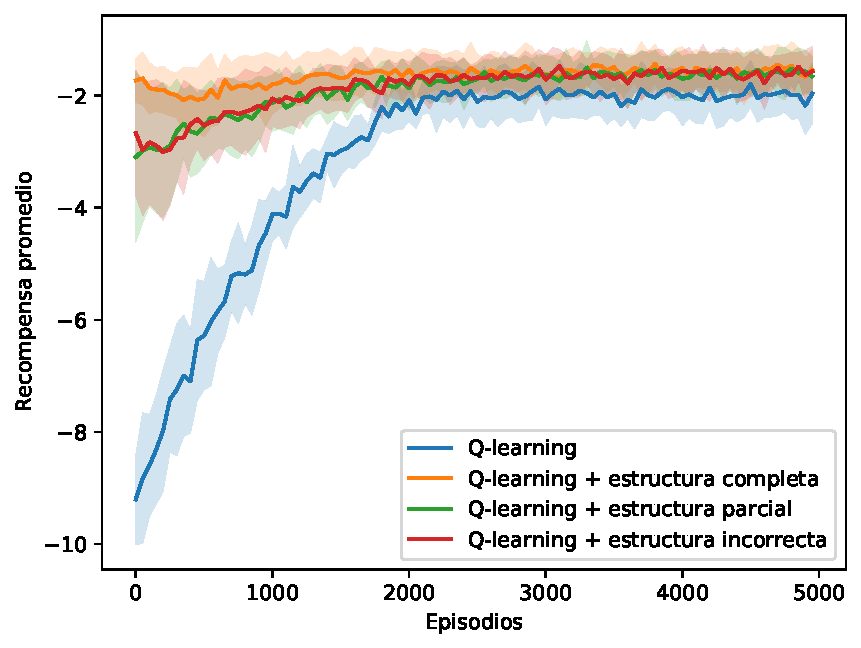
\includegraphics[width=.32\linewidth]{Chapter5/Figs/deltaexp/deterministic_low_025_many_to_one_N_7_experiments_10_episodes_5000_eps_8750.pdf}\\
\rowname{$N = 9$}&
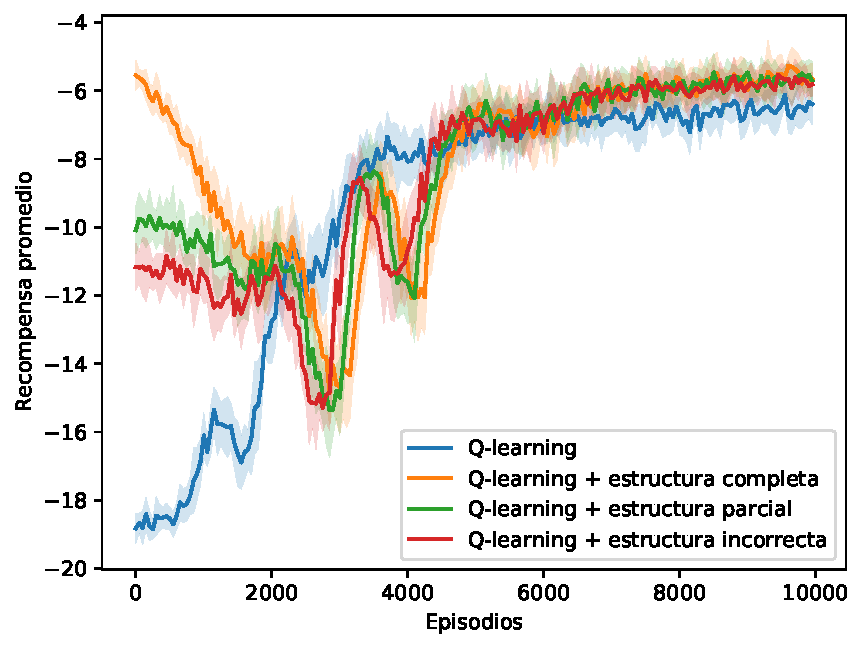
\includegraphics[width=.32\linewidth]{Chapter5/Figs/deltaexp/deterministic_low_025_one_to_one_N_9_experiments_10_episodes_10000_eps_22500.pdf}&
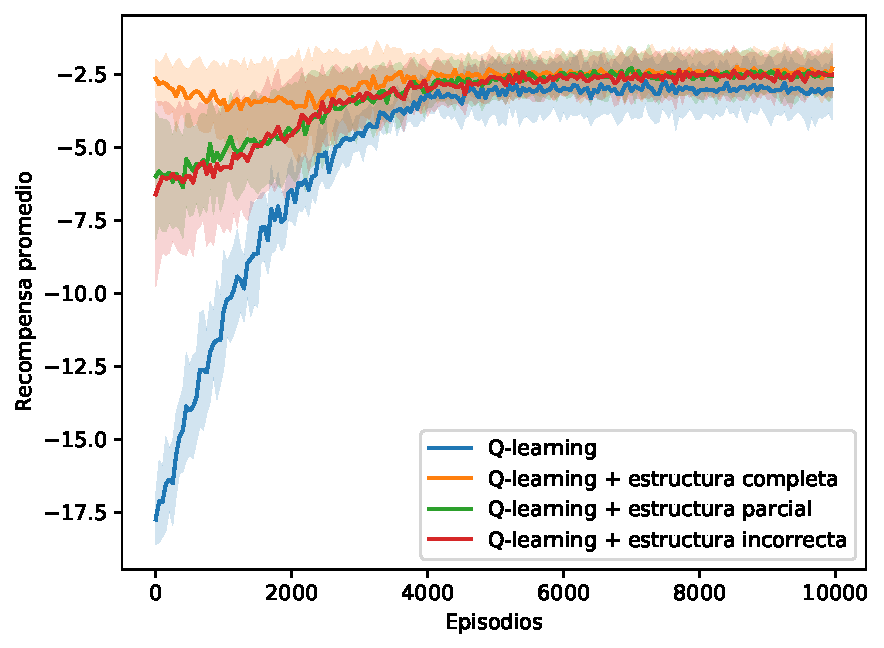
\includegraphics[width=.32\linewidth]{Chapter5/Figs/deltaexp/deterministic_low_025_one_to_many_N_9_experiments_10_episodes_10000_eps_22500.pdf}&
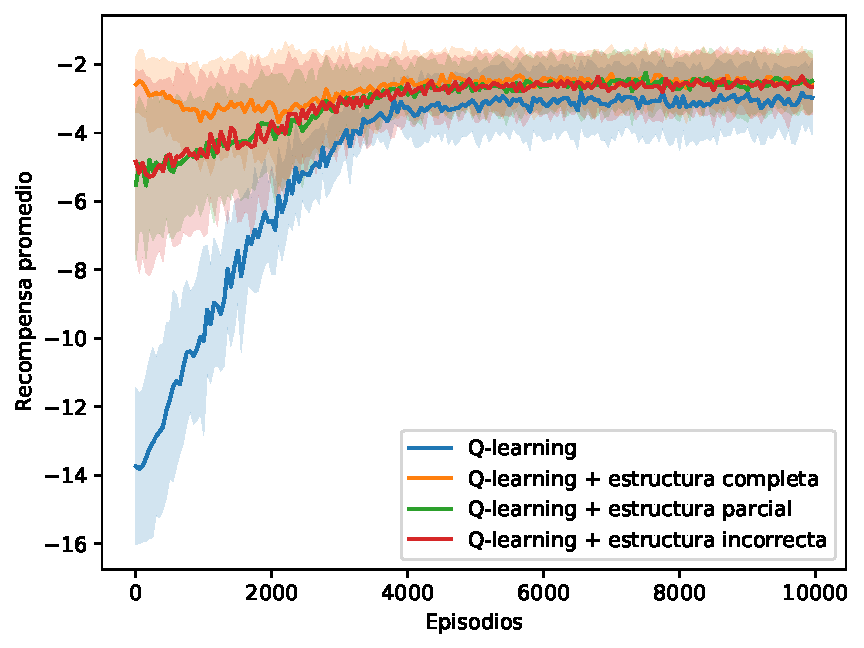
\includegraphics[width=.32\linewidth]{Chapter5/Figs/deltaexp/deterministic_low_025_many_to_one_N_9_experiments_10_episodes_10000_eps_22500.pdf}
\end{tabular}
\caption{Comparación del desempeño para los 4 algoritmos con un nivel de alteración $p_{mod} = 25 \%$  y $\delta = 0.25$ en un ambiente determinista. Las gráficas muestran la medida $average$ y la desviación estándar (región sombreada) para 10 experimentos con 5000 (para $N = 5, 7$) y 10000 (para $N = 9$) episodios.}
\label{fig:low-epsilon-det}
\end{figure}

\newpage

\begin{figure}
\settoheight{\tempdima}{\includegraphics[width=.32\linewidth]{example-image-a}}%
\centering\begin{tabular}{@{}c@{ }c@{ }c@{ }c@{}}
&\textbf{Uno-a-uno} & \textbf{Causa común} & \textbf{Efecto común} \\
\rowname{$N = 5$}&
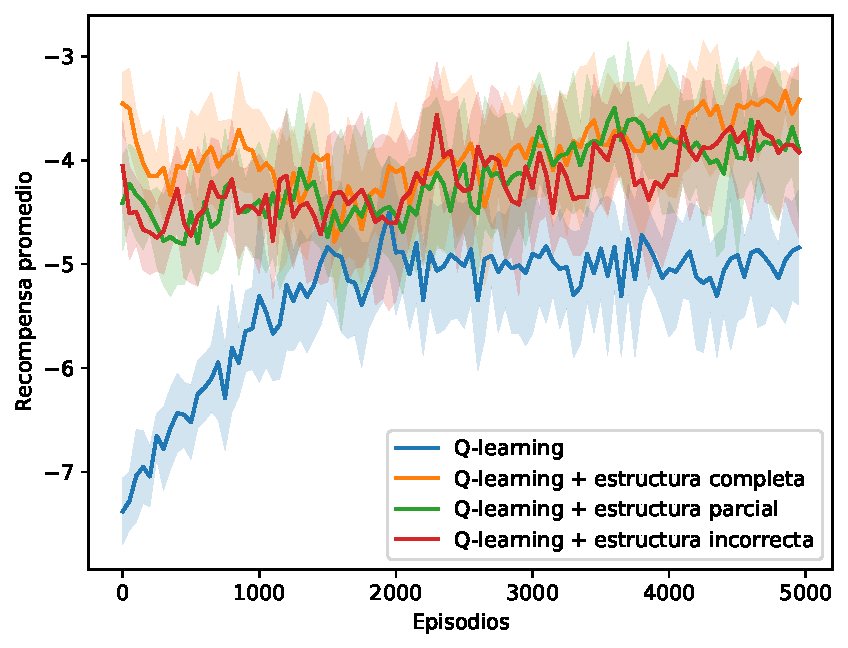
\includegraphics[width=.32\linewidth]{Chapter5/Figs/deltaexp/stochastic_low_025_one_to_one_N_5_experiments_10_episodes_5000_eps_6250.pdf}&
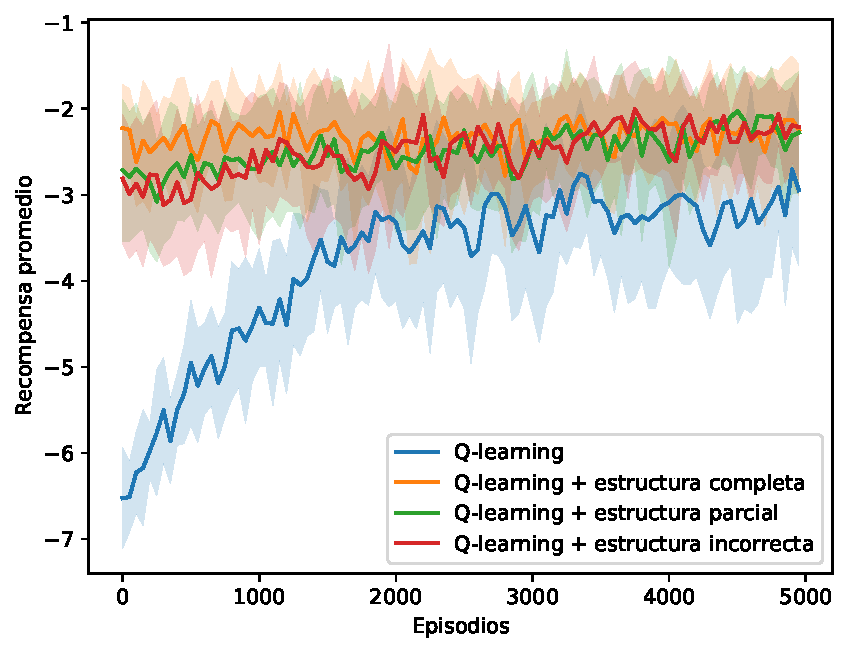
\includegraphics[width=.32\linewidth]{Chapter5/Figs/deltaexp/stochastic_low_025_one_to_many_N_5_experiments_10_episodes_5000_eps_6250.pdf}&
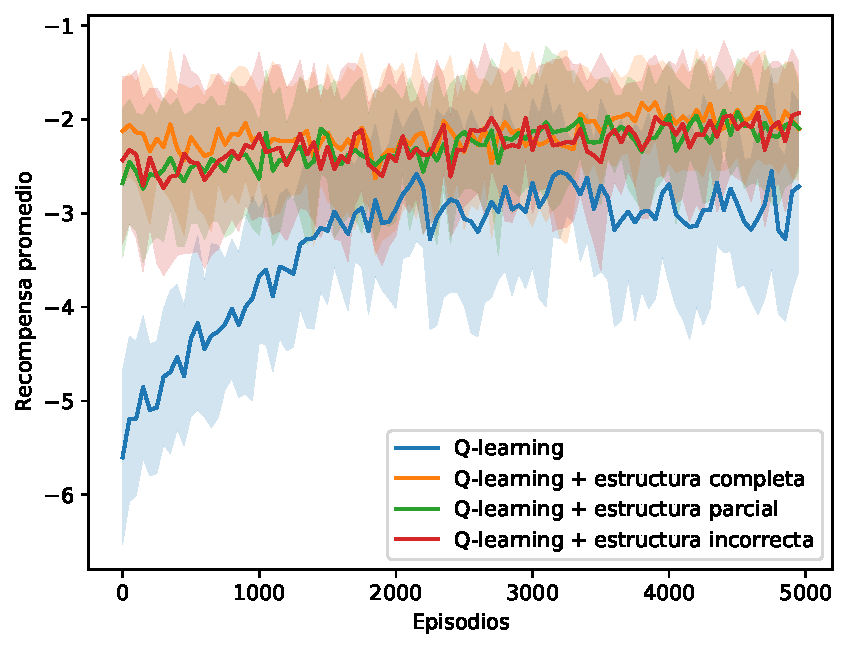
\includegraphics[width=.32\linewidth]{Chapter5/Figs/deltaexp/stochastic_low_025_many_to_one_N_5_experiments_10_episodes_5000_eps_6250.pdf}\\
\rowname{$N=7$}&
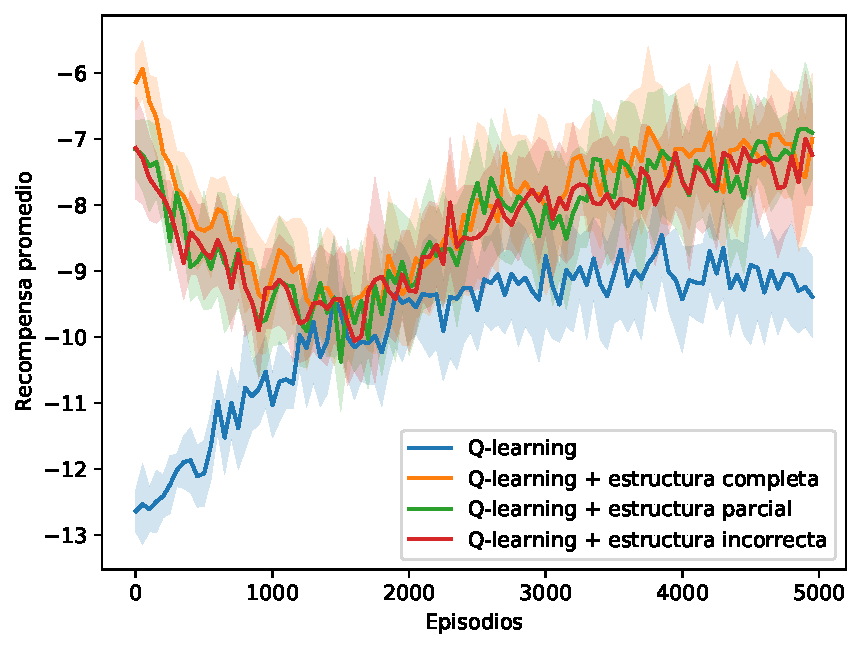
\includegraphics[width=.32\linewidth]{Chapter5/Figs/deltaexp/stochastic_low_025_one_to_one_N_7_experiments_10_episodes_5000_eps_8750.pdf}&
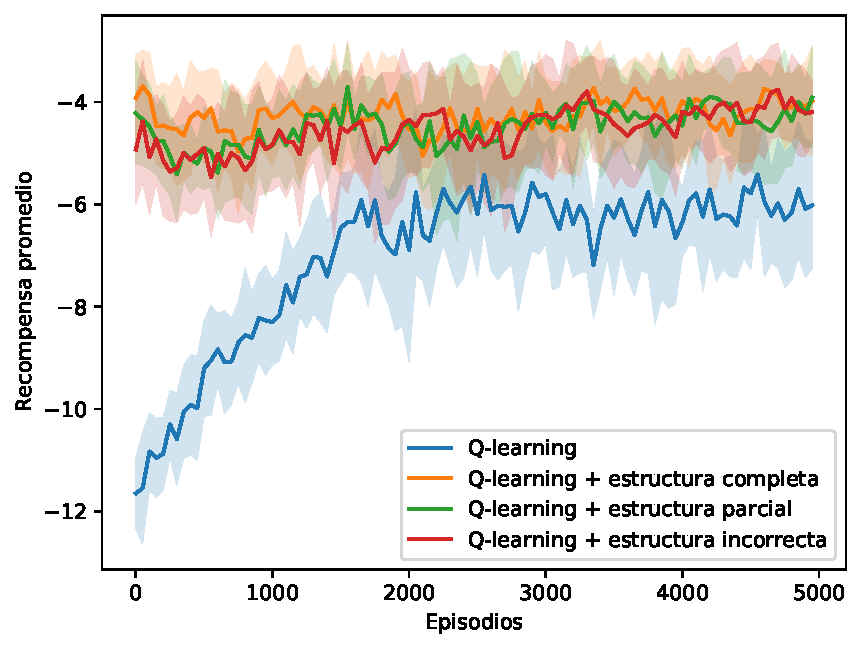
\includegraphics[width=.32\linewidth]{Chapter5/Figs/deltaexp/stochastic_low_025_one_to_many_N_7_experiments_10_episodes_5000_eps_8750.pdf}&
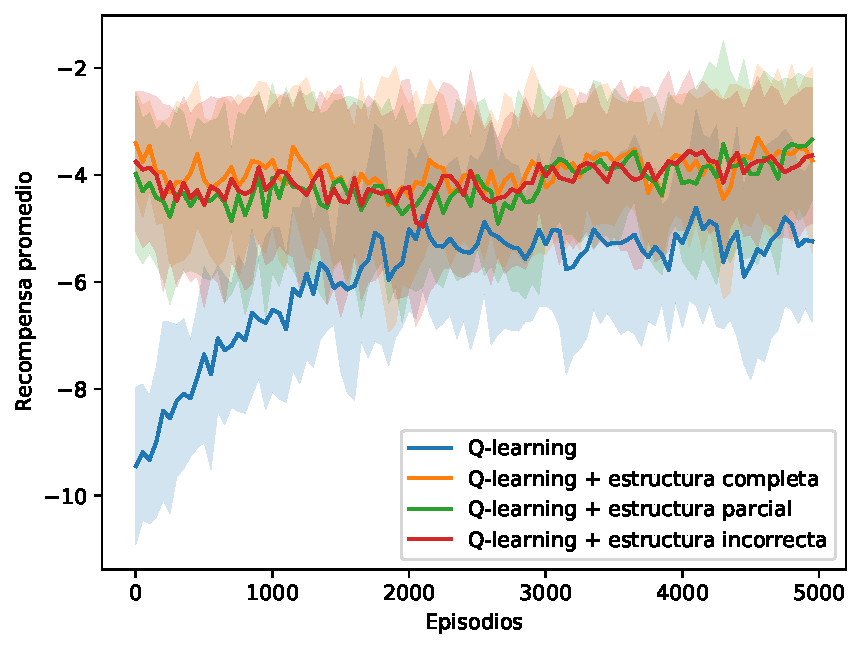
\includegraphics[width=.32\linewidth]{Chapter5/Figs/deltaexp/stochastic_low_025_many_to_one_N_7_experiments_10_episodes_5000_eps_8750.pdf}\\
\rowname{$N = 9$}&
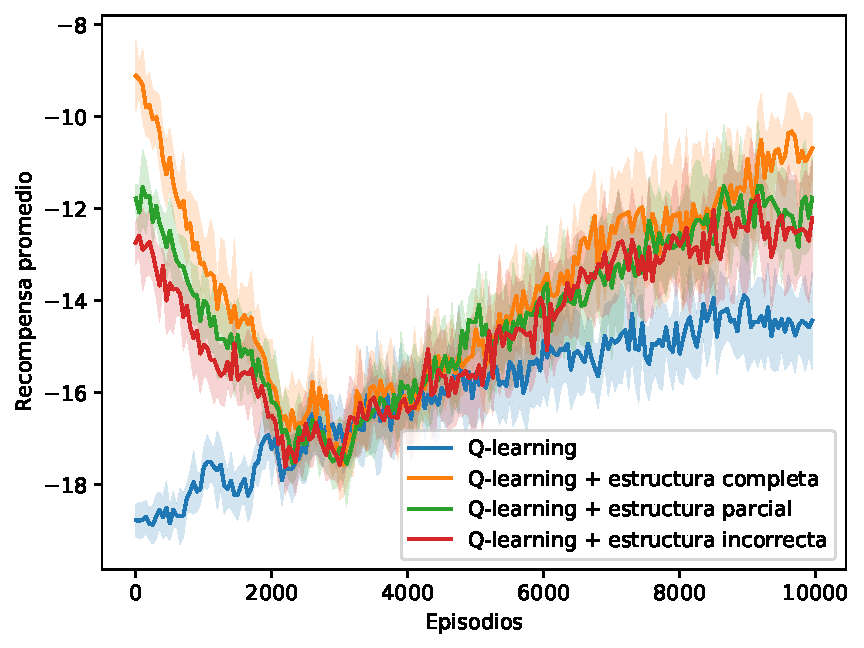
\includegraphics[width=.32\linewidth]{Chapter5/Figs/deltaexp/stochastic_low_025_one_to_one_N_9_experiments_10_episodes_10000_eps_22500.pdf}&
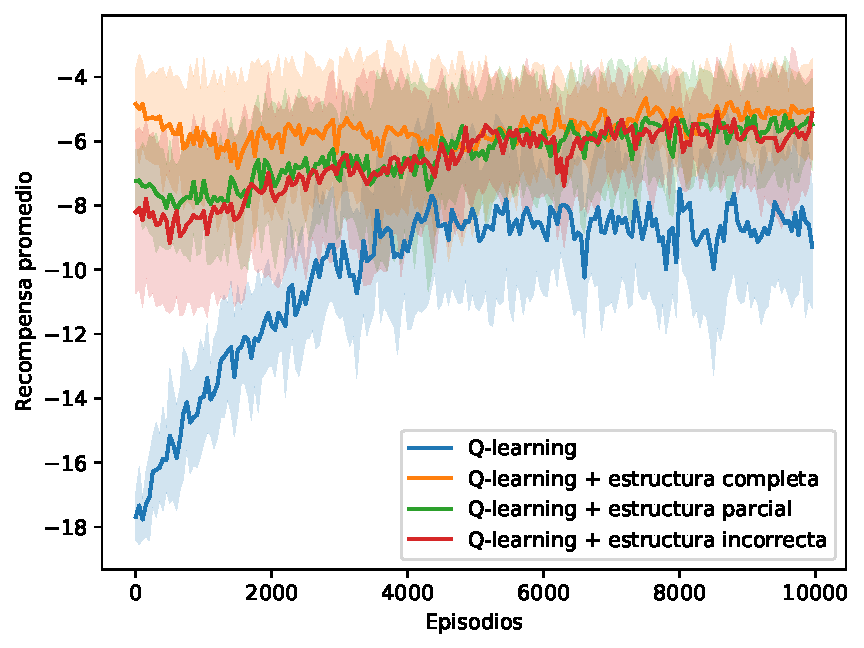
\includegraphics[width=.32\linewidth]{Chapter5/Figs/deltaexp/stochastic_low_025_one_to_many_N_9_experiments_10_episodes_10000_eps_22500.pdf}&
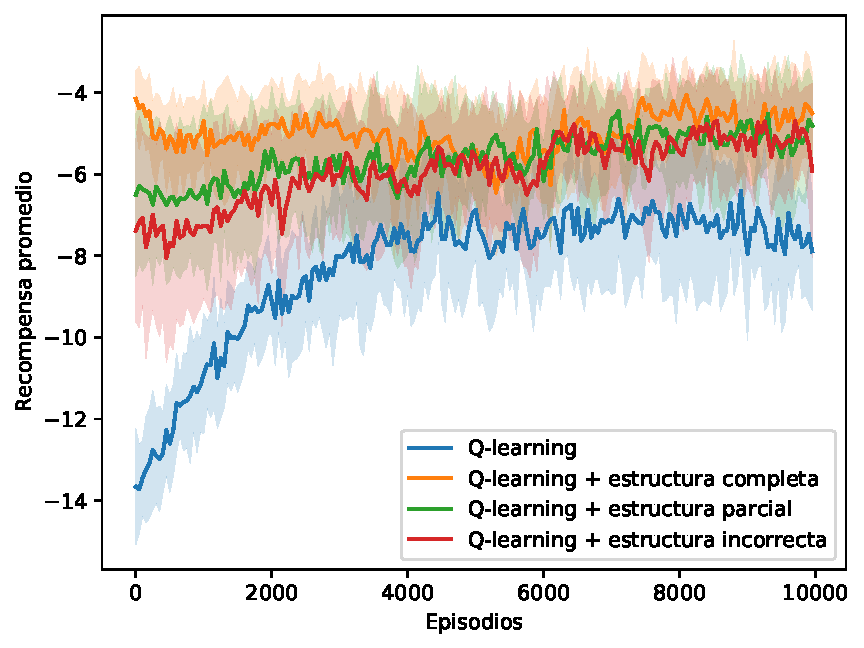
\includegraphics[width=.32\linewidth]{Chapter5/Figs/deltaexp/stochastic_low_025_many_to_one_N_9_experiments_10_episodes_10000_eps_22500.pdf}
\end{tabular}
\caption{Comparación del desempeño para los 4 algoritmos con un nivel de alteración $p_{mod} = 25 \%$  y $\delta = 0.25$ en un ambiente con transiciones estocásticas. Las gráficas muestran la medida $average$ y la desviación estándar (región sombreada)  para 10 experimentos con 5000 (para $N = 5, 7$) y 10000 (para $N = 9$) episodios.}
\label{fig:low-epsilon-sto}
\end{figure}

\newpage

\begin{figure}
\settoheight{\tempdima}{\includegraphics[width=.32\linewidth]{example-image-a}}%
\centering\begin{tabular}{@{}c@{ }c@{ }c@{ }c@{}}
&\textbf{Uno-a-uno} & \textbf{Causa común} & \textbf{Efecto común} \\
\rowname{$N = 5$}&
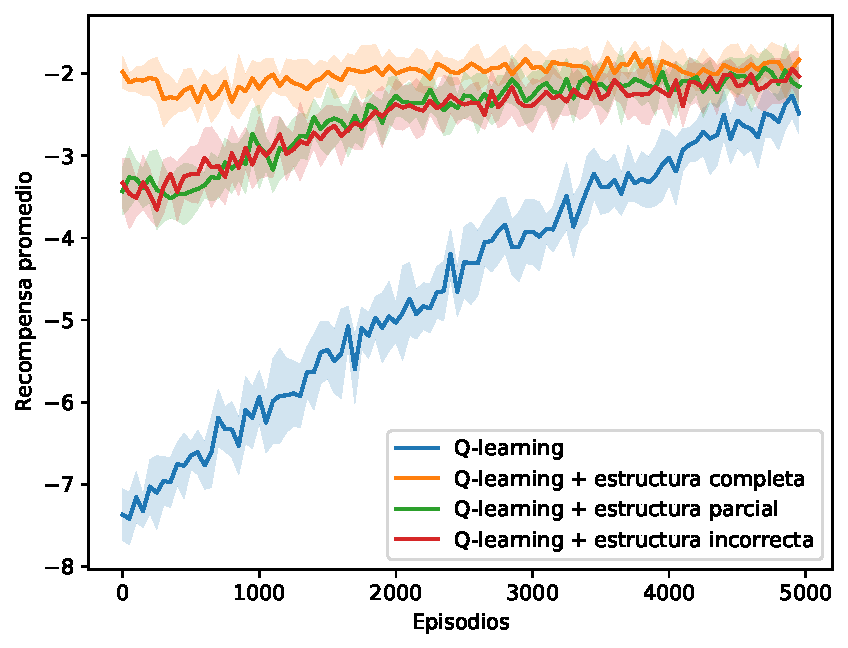
\includegraphics[width=.32\linewidth]{Chapter5/Figs/deltaexp/deterministic_low_025_one_to_one_N_5_experiments_10_episodes_5000_eps_18750.pdf}&
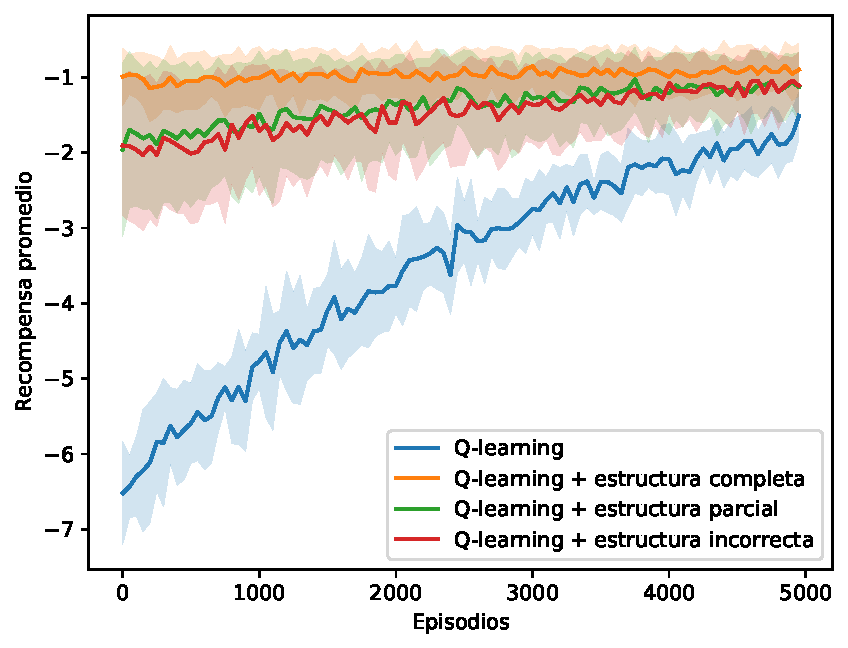
\includegraphics[width=.32\linewidth]{Chapter5/Figs/deltaexp/deterministic_low_025_one_to_many_N_5_experiments_10_episodes_5000_eps_18750.pdf}&
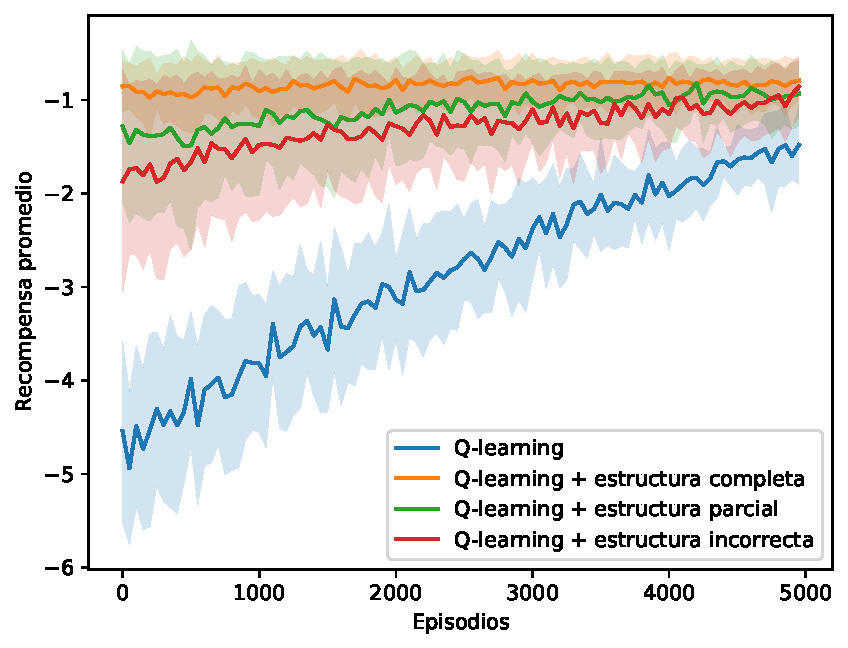
\includegraphics[width=.32\linewidth]{Chapter5/Figs/deltaexp/deterministic_low_025_many_to_one_N_5_experiments_10_episodes_5000_eps_18750.pdf}\\
\rowname{$N=7$}&
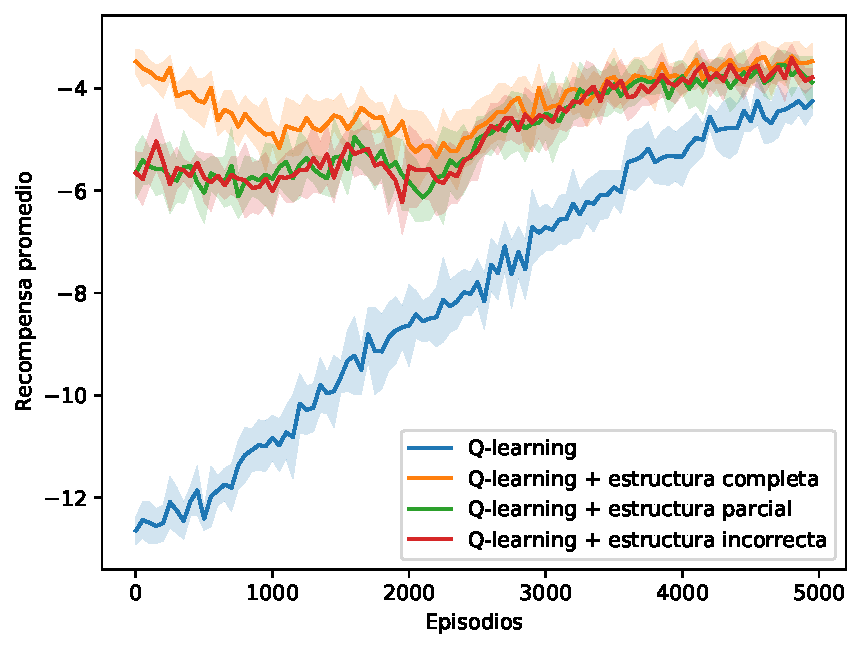
\includegraphics[width=.32\linewidth]{Chapter5/Figs/deltaexp/deterministic_low_025_one_to_one_N_7_experiments_10_episodes_5000_eps_26250.pdf}&
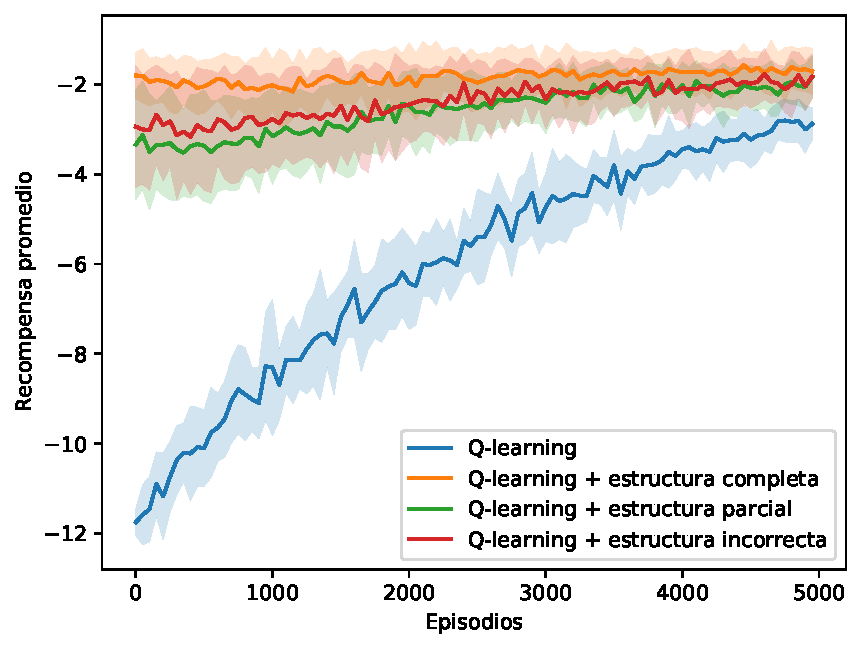
\includegraphics[width=.32\linewidth]{Chapter5/Figs/deltaexp/deterministic_low_025_one_to_many_N_7_experiments_10_episodes_5000_eps_26250.pdf}&
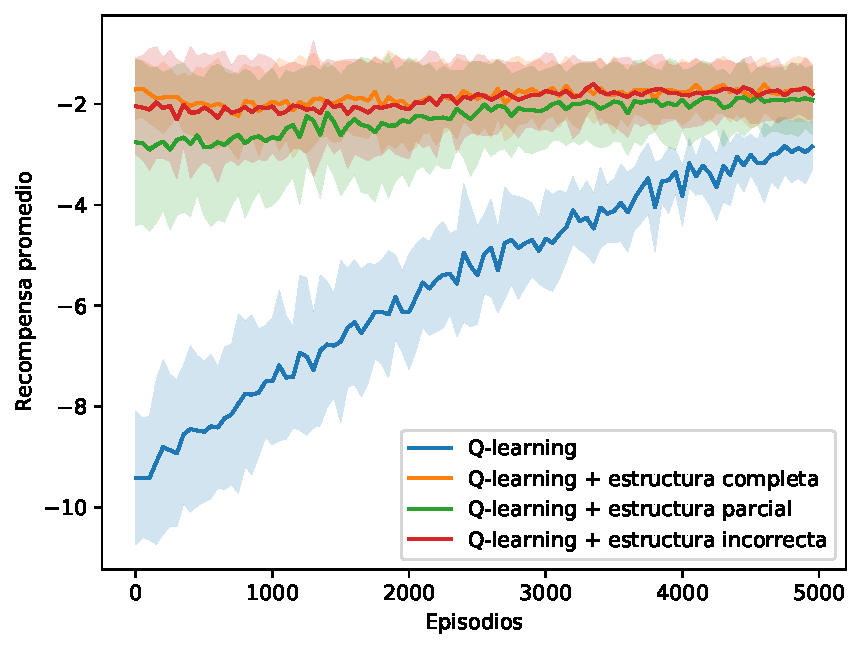
\includegraphics[width=.32\linewidth]{Chapter5/Figs/deltaexp/deterministic_low_025_many_to_one_N_7_experiments_10_episodes_5000_eps_26250.pdf}\\
\rowname{$N = 9$}&
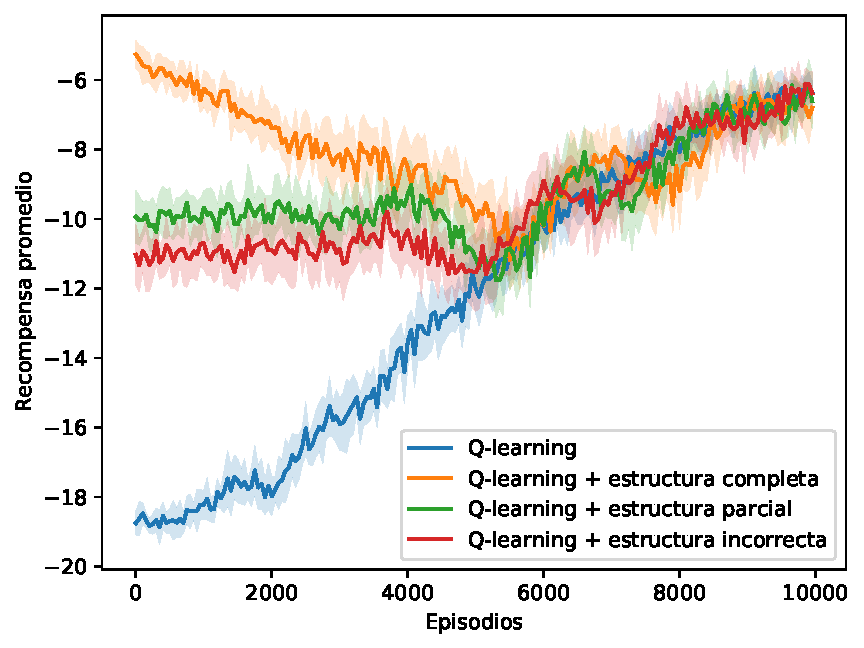
\includegraphics[width=.32\linewidth]{Chapter5/Figs/deltaexp/deterministic_low_025_one_to_one_N_9_experiments_10_episodes_10000_eps_67500.pdf}&
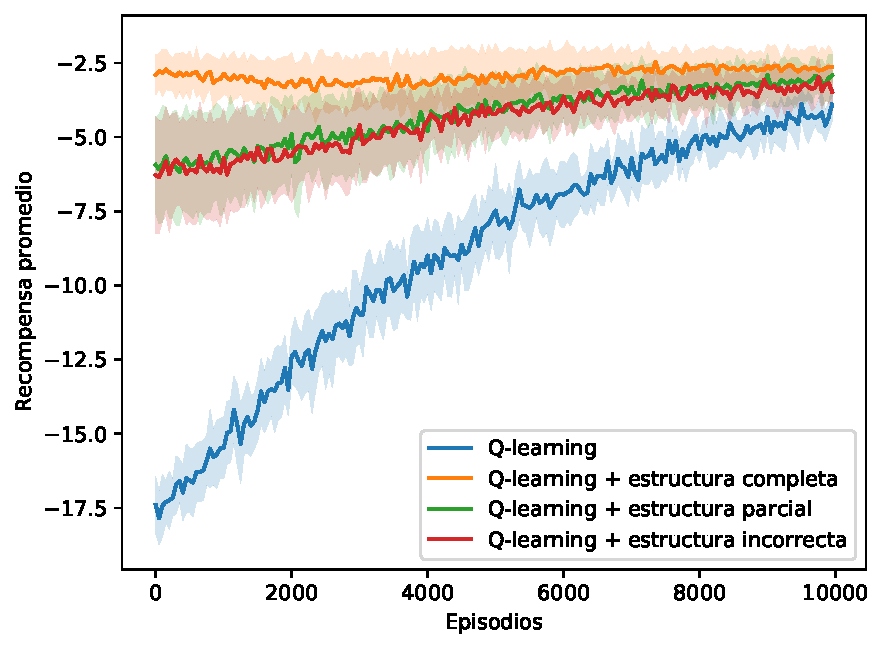
\includegraphics[width=.32\linewidth]{Chapter5/Figs/deltaexp/deterministic_low_025_one_to_many_N_9_experiments_10_episodes_10000_eps_67500.pdf}&
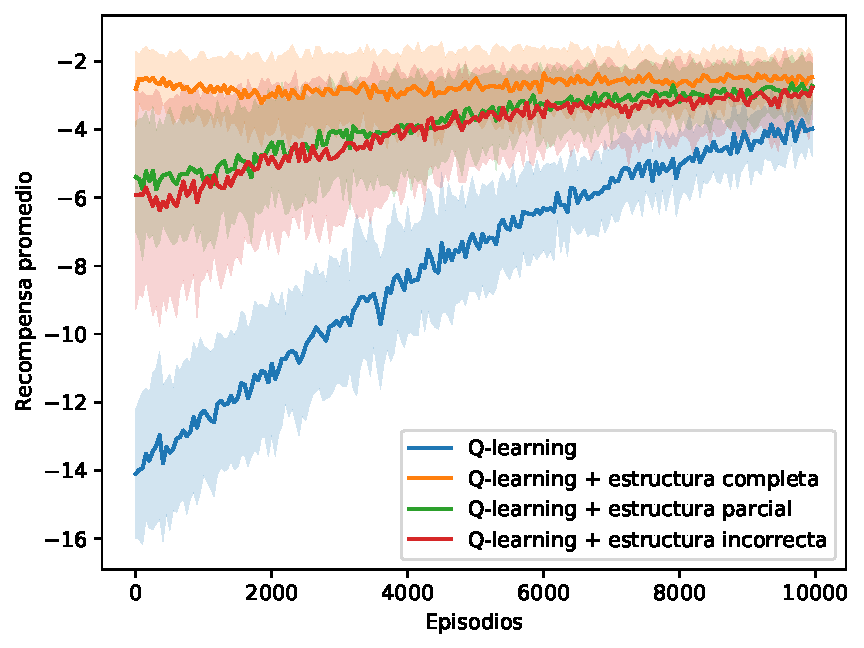
\includegraphics[width=.32\linewidth]{Chapter5/Figs/deltaexp/deterministic_low_025_many_to_one_N_9_experiments_10_episodes_10000_eps_67500.pdf}
\end{tabular}
\caption{Comparación del desempeño para los 4 algoritmos con un nivel de alteración $p_{mod} = 25 \%$ y $\delta = 0.75$ en un ambiente determinista. Las gráficas muestran la medida $average$ y la desviación estándar (región sombreada)  para 10 experimentos con 5000 (para $N = 5, 7$) y 10000 (para $N = 9$) episodios.}
\label{fig:high-epsilon-det}
\end{figure}

\newpage

\begin{figure}
\settoheight{\tempdima}{\includegraphics[width=.32\linewidth]{example-image-a}}%
\centering\begin{tabular}{@{}c@{ }c@{ }c@{ }c@{}}
&\textbf{Uno-a-uno} & \textbf{Causa común} & \textbf{Efecto común} \\
\rowname{$N = 5$}&
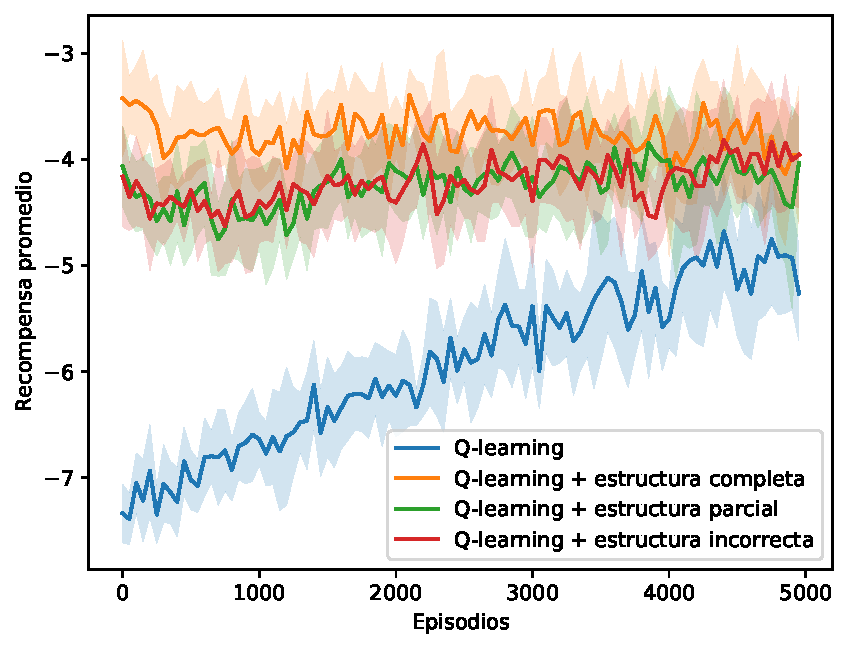
\includegraphics[width=.32\linewidth]{Chapter5/Figs/deltaexp/stochastic_low_025_one_to_one_N_5_experiments_10_episodes_5000_eps_18750.pdf}&
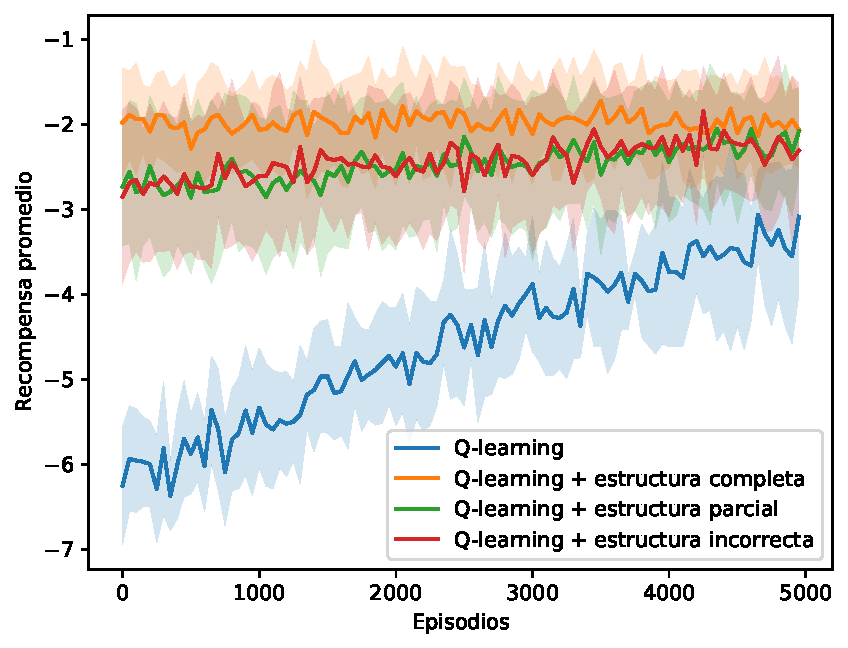
\includegraphics[width=.32\linewidth]{Chapter5/Figs/deltaexp/stochastic_low_025_one_to_many_N_5_experiments_10_episodes_5000_eps_18750.pdf}&
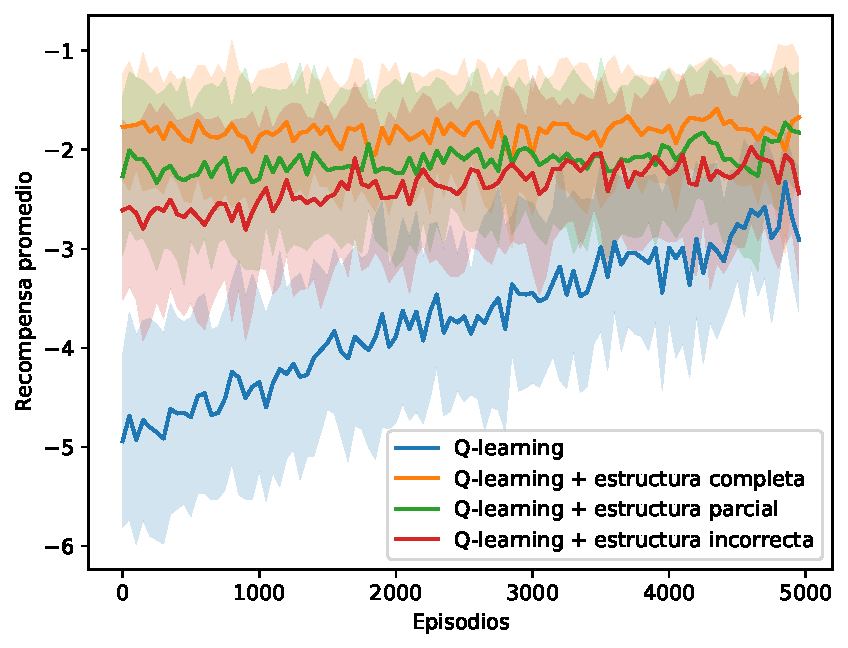
\includegraphics[width=.32\linewidth]{Chapter5/Figs/deltaexp/stochastic_low_025_many_to_one_N_5_experiments_10_episodes_5000_eps_18750.pdf}\\
\rowname{$N=7$}&
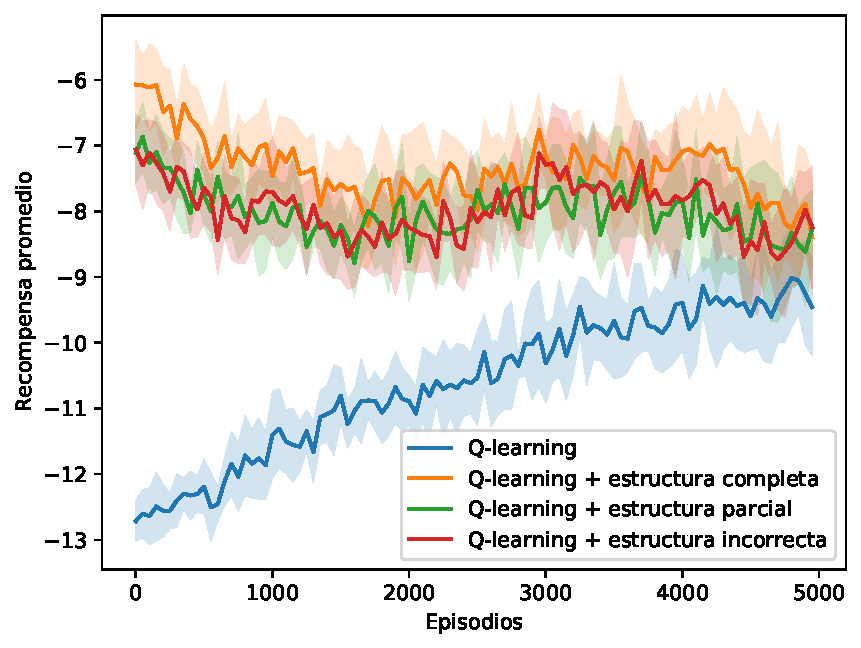
\includegraphics[width=.32\linewidth]{Chapter5/Figs/deltaexp/stochastic_low_025_one_to_one_N_7_experiments_10_episodes_5000_eps_26250.pdf}&
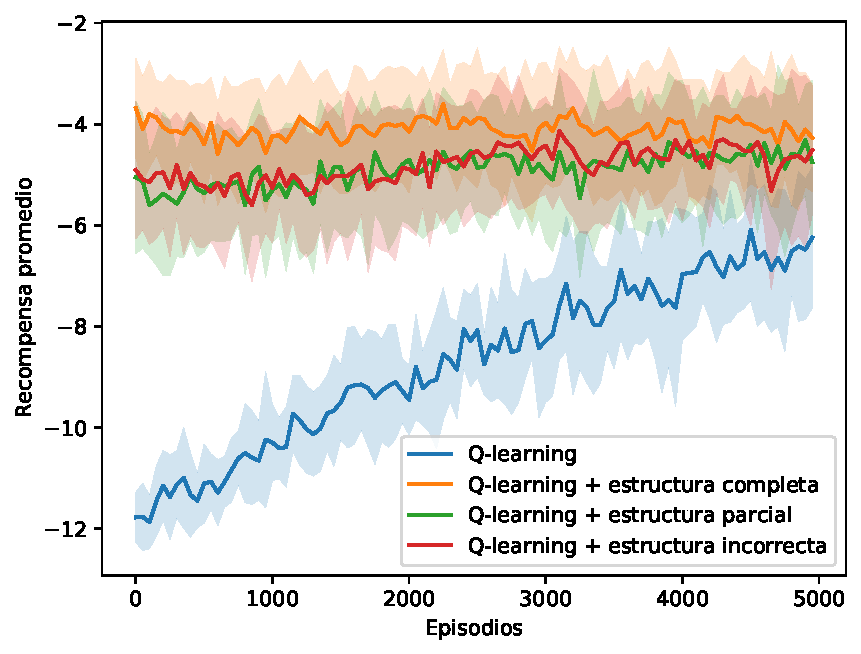
\includegraphics[width=.32\linewidth]{Chapter5/Figs/deltaexp/stochastic_low_025_one_to_many_N_7_experiments_10_episodes_5000_eps_26250.pdf}&
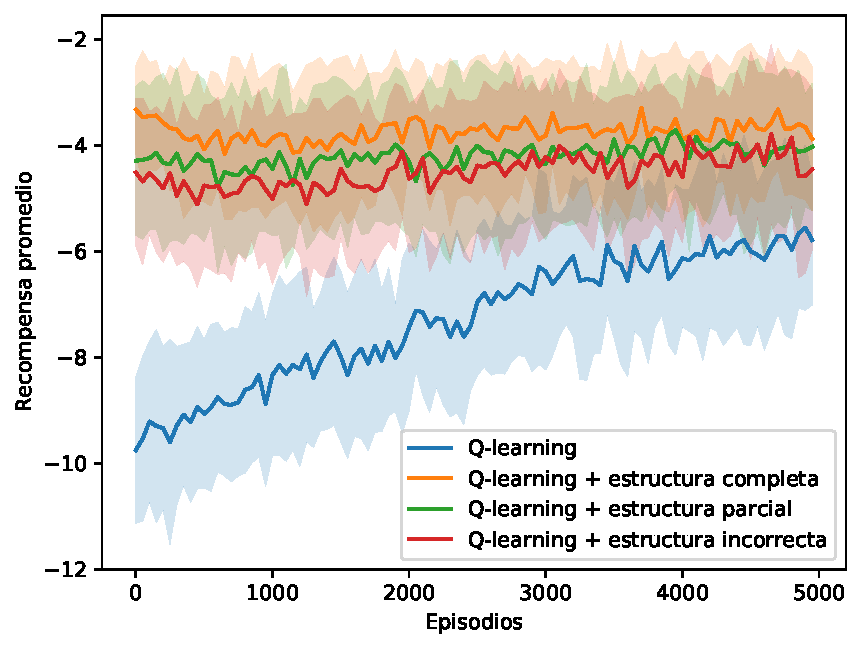
\includegraphics[width=.32\linewidth]{Chapter5/Figs/deltaexp/stochastic_low_025_many_to_one_N_7_experiments_10_episodes_5000_eps_26250.pdf}\\
\rowname{$N = 9$}&
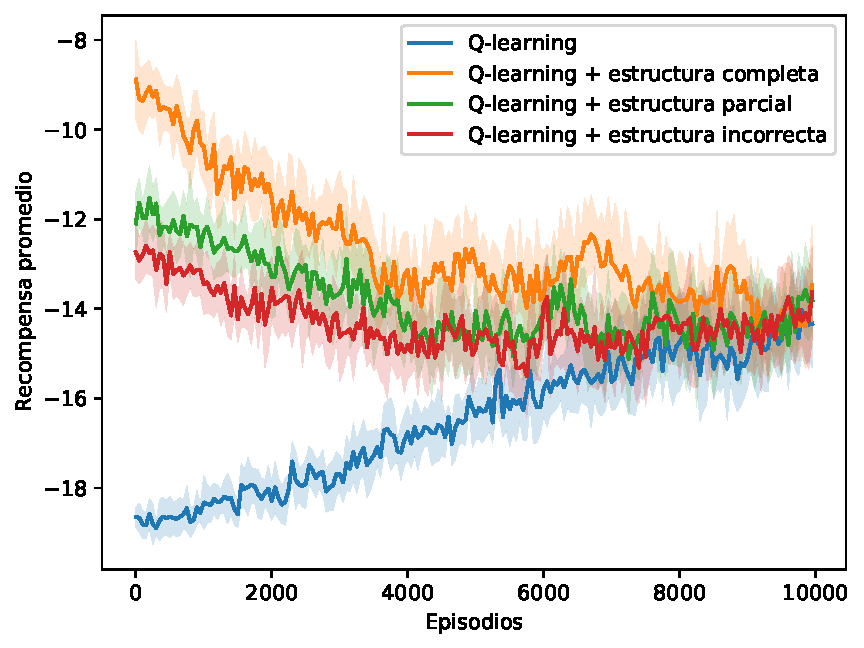
\includegraphics[width=.32\linewidth]{Chapter5/Figs/deltaexp/stochastic_low_025_one_to_one_N_9_experiments_10_episodes_10000_eps_67500.pdf}&
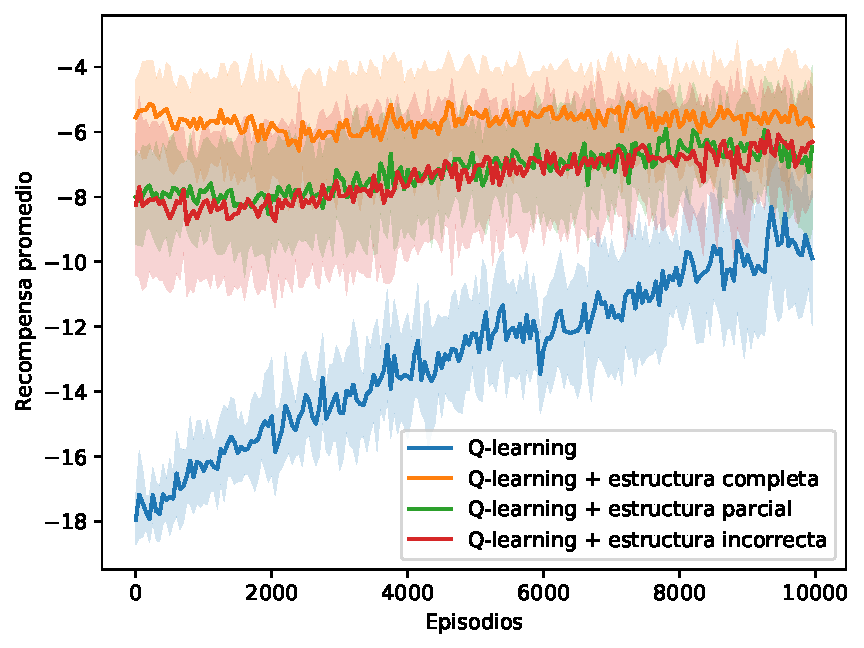
\includegraphics[width=.32\linewidth]{Chapter5/Figs/deltaexp/stochastic_low_025_one_to_many_N_9_experiments_10_episodes_10000_eps_67500.pdf}&
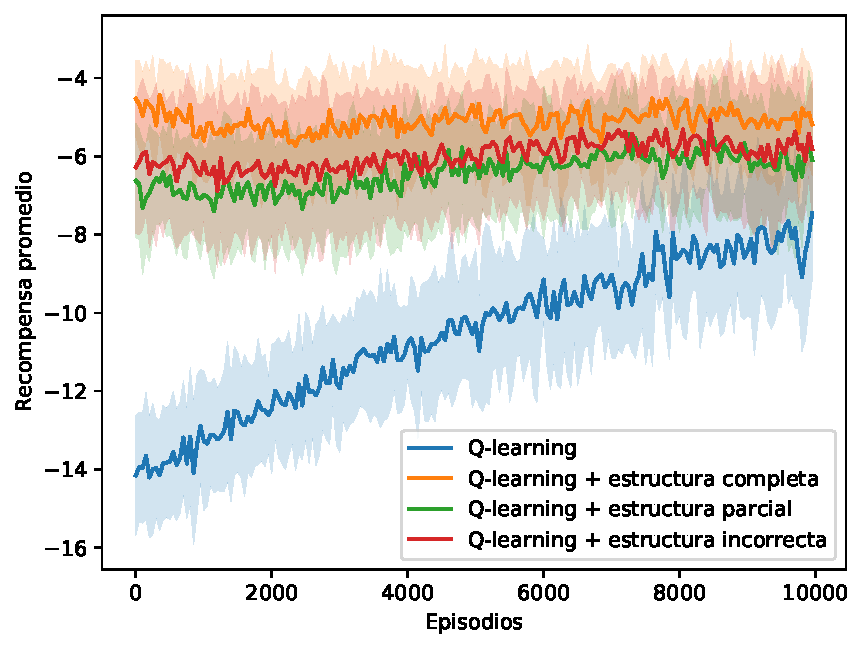
\includegraphics[width=.32\linewidth]{Chapter5/Figs/deltaexp/stochastic_low_025_many_to_one_N_9_experiments_10_episodes_10000_eps_67500.pdf}
\end{tabular}
\caption{Comparación del desempeño para los 4 algoritmos con un nivel de alteración $p_{mod} = 25 \%$ y $\delta = 0.75$ en un ambiente estocástico. Las gráficas muestran la medida $average$ y la desviación estándar (región sombreada) para 10 experimentos con 5000 (para $N = 5, 7$) y 10000 (para $N = 9$) episodios.}
\label{fig:high-epsilon-sto}
\end{figure}

